\setAuthor{Eero Vaher}
\setRound{lõppvoor}
\setYear{2015}
\setNumber{G 5}
\setDifficulty{5}
\setTopic{Kinemaatika}

\prob{Pallivise}
Juku elab silindrikujulises kosmosejaamas, mille pöörlemine tekitab kunstliku raskusjõu. Jaama raadius on $R$, selle pöörlemise nurkkiirus $\omega$. Juku viskab palli otse üles algkiirusega $v=\frac{\sqrt{3}}{3}\omega R$. Kui kaugele Jukust mööda jaama pinda pall maandub?

\hint
Palli lendu on mugav vaadelda laboratoorses taustsüsteemis. Sellisel juhul liigub pall pärast viset ühtlaselt ning sirgjooneliselt, kusjuures selle kiiruse vertikaalsihiline komponent on $v$ ning horisontaalsihiline komponent $\omega R$.

\solu
Vaatleme palli lendu jaama teljega seotud inertsiaalses taustsüsteemis. Olgu Juku koordinaadid palli viskamise hetkel $(0,-R)$. Sellisel juhul liigub pall pärast viset ühtlaselt ning sirgjooneliselt, kusjuures selle kiiruse vertikaalsihiline komponent on $v$ ning horisontaalsihiline komponent $\omega R$. Järelikult $\tan\alpha=\frac{\omega R}{v}$, millest saame $\alpha=\frac{\pi}{3}$. Kuna kehtib $\varphi=\pi-2\alpha$, siis saame järeldada, et ka $\varphi=\frac{\pi}{3}$ ning pall läbib enne jaama pinnani jõudmist teepikkuse $R$. Palli kiirus on
\[
\sqrt{v^2+\omega^2R^2}=\frac{2\sqrt{3}}{3}\omega R,
\]
seega on pall õhus aja $t=\frac{\sqrt{3}}{2\omega}$, mille jooksul jõuab jaam pöörduda nurga $\theta=\omega t=\frac{\sqrt{3}}{2}$ võrra. Järelikult näeb Juku otse üles visatud palli maanduvat enda ees kaugusel
\[
\left(\varphi-\theta\right)R=\left(\frac{\pi}{3}-\frac{\sqrt{3}}{2}\right)R.
\]

\begin{center}
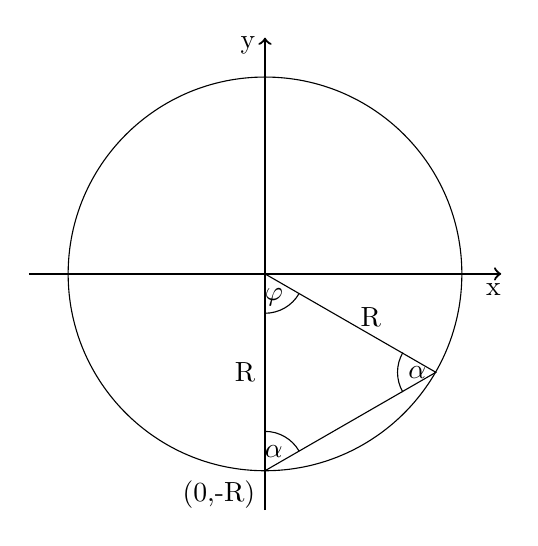
\begin{tikzpicture}[scale=1]
\draw (2.5,0) arc (0:360:2.5);
\draw[->,thick] (-3,0) -- (3,0);
\node[below] at (2.9,0) {x};
\draw[->,thick] (0,-3) -- (0,3);
\node[left] at (0,2.9) {y};
\node[left] at (0,-2.8) {(0,-R)};
\draw (0,-2.5) -- (2.17,-1.25) -- (0,0);
\node[right] at (-0.125,-2.25) {$\alpha$};
\draw (0,-2) arc (90:30:0.5);
\node[left] at (2.17,-1.25) {$\alpha$};
\draw (1.75, -1.5) arc (210:150:0.5);
\node[right] at (-0.125,-0.3) {$\varphi$};
\draw (0,-0.5) arc (270:330:0.5);
\node[left] at (0,-1.25) {R};
\node[right] at (1.09,-0.55) {R};
\end{tikzpicture}
\end{center}

\probeng{Ball throw}
Juku is living in a cylindrical space station that rotates so that artificial gravitational force is created. The radius of the station is $R$, its rotation’s angular velocity is $\omega$. Juku throws a ball straight up with an initial speed $v=\frac{\sqrt{3}}{3}\omega R$. From how far away from Juku along the surface of the station will the ball land?

\hinteng
It is convenient to observe the flight of the ball in the laboratory frame of reference. In this case the ball moves linearly and uniformly after the throw, moreover its velocity’s vertical component is $v$ and horizontal component $\omega R$.

\solueng
Let us observe the flight of the ball in the station’s inertial frame of reference. Let Juku’s coordinates at the moment of throwing the ball be $(0,-R)$. In this case the ball moves uniformly and along a straight line, moreover the vertical component of this velocity is $v$ and horizontal component $\omega R$. Therefore $\tan\alpha=\frac{\omega R}{v}$ from which we get $\alpha=\frac{\pi}{3}$. Because $\varphi=\pi-2\alpha$ applies we can conclude that also $\varphi=\frac{\pi}{3}$ and the ball covers the distance $R$ before reaching the station’s surface. The ball’s velocity is $\sqrt{v^2+\omega^2R^2}=\frac{2\sqrt{3}}{3}\omega R$ therefore the ball is in the air for the time $t=\frac{\sqrt{3}}{2\omega}$ during which the station has managed to turn by an angle $\theta=\omega t=\frac{\sqrt{3}}{2}$. Thus, Juku sees a ball that is thrown directly up land at a distance $\left(\varphi-\theta\right)R=\left(\frac{\pi}{3}-\frac{\sqrt{3}}{2}\right)R$ from him.
\begin{center}
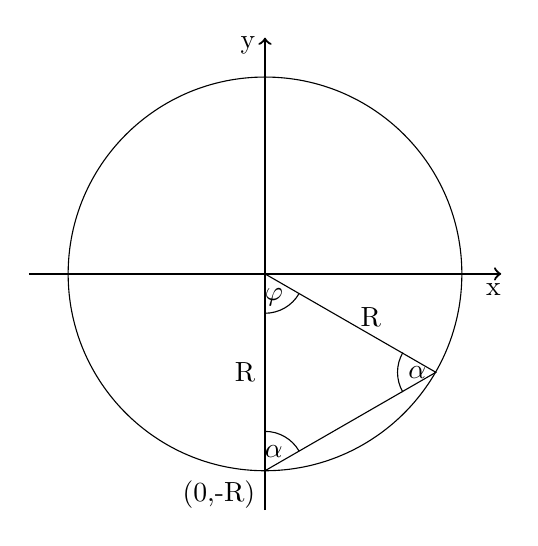
\begin{tikzpicture}[scale=1]
\draw (2.5,0) arc (0:360:2.5);
\draw[->,thick] (-3,0) -- (3,0);
\node[below] at (2.9,0) {x};
\draw[->,thick] (0,-3) -- (0,3);
\node[left] at (0,2.9) {y};
\node[left] at (0,-2.8) {(0,-R)};
\draw (0,-2.5) -- (2.17,-1.25) -- (0,0);
\node[right] at (-0.125,-2.25) {$\alpha$};
\draw (0,-2) arc (90:30:0.5);
\node[left] at (2.17,-1.25) {$\alpha$};
\draw (1.75, -1.5) arc (210:150:0.5);
\node[right] at (-0.125,-0.3) {$\varphi$};
\draw (0,-0.5) arc (270:330:0.5);
\node[left] at (0,-1.25) {R};
\node[right] at (1.09,-0.55) {R};
\end{tikzpicture}
\end{center}
\probend